%% ****** Start of file aiptemplate.tex ****** %
%%
%%   This file is part of the files in the distribution of AIP substyles for REVTeX4.
%%   Version 4.1 of 9 October 2009.
%%
%
% This is a template for producing documents for use with 
% the REVTEX 4.1 document class and the AIP substyles.
% 
% Copy this file to another name and then work on that file.
% That way, you always have this original template file to use.

%\documentclass[aip,graphicx]{revtex4-1}
%\documentclass[aip,reprint]{revtex4-1}

%\usepackage{graphicx}

%\draft % marks overfull lines with a black rule on the right
%\documentclass[pre,aps,floatfix,authordate1-4,twocolumn]{revtex4-1}
%\documentclass[pre,aps,floatfix,authordate1-4]{revtex4-1}

\documentclass[aps,prl,superscriptaddress,twocolumn]{revtex4}



%\documentclass[aps,prl,preprint,groupedaddress]{revtex4}

\usepackage{rotating} 
\usepackage{times}
\usepackage{graphicx}
\usepackage{setspace}
\usepackage{amsmath}
\usepackage{epstopdf}
\usepackage[obeyFinal]{easy-todo}
\begin{document}

% Use the \preprint command to place your local institutional report number 
% on the title page in preprint mode.
% Multiple \preprint commands are allowed.
%\preprint{}

\title{NMRlipids IV: Other than PC headgroups} %Title of paper

% repeat the \author .. \affiliation  etc. as needed
% \email, \thanks, \homepage, \altaffiliation all apply to the current author.
% Explanatory text should go in the []'s, 
% actual e-mail address or url should go in the {}'s for \email and \homepage.
% Please use the appropriate macro for the type of information

% \affiliation command applies to all authors since the last \affiliation command. 
% The \affiliation command should follow the other information.

\author{O. H. Samuli Ollila}
\email[]{samuli.ollila@helsinki.fi}
%\homepage[]{Your web page}
%\thanks{}
%\altaffiliation{}
\affiliation{University of Helsinki}


% Collaboration name, if desired (requires use of superscriptaddress option in \documentclass). 
% \noaffiliation is required (may also be used with the \author command).
%\collaboration{}
%\noaffiliation

\date{\today}

\begin{abstract}
% insert abstract here
  Primarily measured but also simulated NMR order parameters will be collected also for other than phophatidylcholine
  (these are discussed in NMRlipids I) headgroup. The information will be used to understand structural differences between different lipid molecules in bilayers.
\end{abstract}

%\pacs{}% insert suggested PACS numbers in braces on next line

\maketitle %\maketitle must follow title, authors, abstract and \pacs

% Body of paper goes here. Use proper sectioning commands. 
% References should be done using the \cite, \ref, and \label commands


%\label{}
\section{Introduction}
Primarily measured but also simulated NMR order parameters will be collected also for other than phophatidylcholine (these are discussed in NMRlipids I) headgroup. The information will be used to understand structural differences between different lipid molecules in bilayers.

%\section{Methods}

%\subsection{Molecular dynamics simulations}

\section{Comparison of order parameters between different headgroups}

Experimental order parameters for different lipid headgroups are
collected in Fig. \ref{HGorderParameters}.
\begin{figure}[]
  \centering
  \includegraphics[width=17.2cm]{../Figs/HGorderparameters.eps}
  \caption{\label{HGorderParameters}
    Order parameters for headgroup and glycerol backbone with different headgroups
  }
\end{figure}

\section{Ion binding in bilayers with charged lipids}

Headgroup order parameters as a function of CaCl concentration
from experiments with charged lipids are shown in Figs \ref{OrderParametersWithCaCl}
and \ref{OrderParametersWithCaClBELOW1M}.

Order parameter changes are shown in Fig. \ref{OrderParameterCHANGESWithCaClBELOW1M}

\begin{figure}[]
  \centering
  \includegraphics[width=17.2cm]{../Figs/LIPIDSwithCaCl.eps}
  \caption{\label{OrderParametersWithCaCl}
    PC headgroup order parameters as a function of CaCl concentration for systems with charged lipids.
  }
\end{figure}
\begin{figure}[]
  \centering
  \includegraphics[width=17.2cm]{../Figs/LIPIDSwithCaClBELOW1M.eps}
  \caption{\label{OrderParametersWithCaClBELOW1M}
    Figure \ref{OrderParametersWithCaCl} zoomed to smaller concentrations.
  }
\end{figure}


\begin{figure}[]
  \centering
  \includegraphics[width=17.2cm]{../Figs/CHANGESwithCaClBELOW1M.eps}
  \caption{\label{OrderParameterCHANGESWithCaClBELOW1M}
    Changes in order parameters
  }
\end{figure}




\section{Conclusions}

% Tables may be be put in the text as floats.
% Here is an example of the general form of a table:
% Fill in the caption in the braces of the \caption{} command. Put the label
% that you will use with \ref{} command in the braces of the \label{} command.
% Insert the column specifiers (l, r, c, d, etc.) in the empty braces of the
% \begin{tabular}{} command.
%
% \begin{table}
% \caption{\label{} }
% \begin{tabular}{}
% \end{tabular}
% \end{table}

% If you have acknowledgments, this puts in the proper section head.
\begin{acknowledgments}
% Put your acknowledgments here.
\end{acknowledgments}
\newpage
\appendix
\begin{center}
{\bf SUPPLEMENTARY INFORMATION}
\end{center}


% Create the reference section using BibTe
\bibliography{refs.bib}

%\newpage
%\section{APPENDIX: The NMR results reported by Tiago Ferreira}

\listoftodos

\end{document}
%
% ****** End of file aiptemplate.tex ******
